
% JuliaCon proceedings template
\documentclass{juliacon}[12pt]
\setcounter{page}{1}
\usepackage[utf8]{inputenc}

%\newcommand{\pkg}[1]{{\it #1}}
\newcommand{\pkg}[1]{{\small \textsc{#1}}}
\newcommand{\struct}[1]{{\it {#1}}}
\newcommand{\tbd}{}

\begin{document}

\title{Digital Twins for Ocean Robots}

\author[1]{Gaël Forget}
\affil[1]{Earth, Atmospheric and Planetary Sciences, Massachusetts Institute of Technology, \newline
77 Massachusetts Avenue, Cambridge, 02139, MA, USA}

\keywords{Julia, Ocean, Climate, Robot, Observation, Observing, Platform, Sensor, Drifter, Buoy, Profiler, Model, Modeling, Machine Learning, Artificial Intelligence, Data Assimilation, Parameter Inference, Climatology, Geospatial, Statistics}

\hypersetup{
pdftitle = {Digital Twins for Ocean Robot},
pdfsubject = {JuliaCon 2023 Proceedings},
pdfauthor = {Gaël Forget},
pdfkeywords = {Julia, Ocean, Robots, Observation, In Situ, Model},
}

\maketitle

\begin{abstract}

DTOR is a framework to access, analyze, and simulate the global fleet of ocean observing devices (or {\it ocean robots}) that monitor climate change. It brings these observations to Julia and lets us pair ocean robots with virtual counterparts (or {\it twins}). Digital twins provide a bridge from the data to predictive models and enable machine learning. In turn, observing system simulations in a digital environment can help evaluate observational strategies a priori, during deployment, or afterwards. In this paper we present the DTOR framework, its supported observing systems, capabilities to simulate ocean robots, and envisioned applications. 

%A fleet of ocean robots is collecting data that are crucial to monitor, understand, and predict climate change. Our {\it digital twins for ocean robots} framework brings these data to Julia and provides the ability to pair them with a virtual counterpart. The simulated ocean robots provide a bridge to numerical models and enable machine learning. In turn, the simulated observation of a virtual Earth can be used to evaluate observing system strategies ahead a priori, and once they are in operation. Our frameworks can readily simulates complex data sets being collected at sea. It leverages multiple Julia packages developed by the author and the community. The 2023 JuliaCon talk focused on the global observing system being simulated, as well as the expected scientific, societal, and commercial applications.

\end{abstract}

\section{Introduction}

The DTOR framework was introduced at the Symposium on Advances in Ocean Observation in 2022, and later presented to US-CLIVAR and JuliaCon in 2023, and the OceanPredict Symposium in 2024. The primary goal of DTOR is to associate ocean observing systems (or {\it ocean robots}) with virtual counterparts (or {\it twins}), and do it for the whole fleet of ocean robots that are currently at sea or have observed the Ocean in the past (Fig.~\ref{fig:ocean-ops}). The virtual twins are to be created through numerical model simulations, which can come in different flavors and languages. The simulation of observing systems in the future, as climate change progresses, is also part of the scope of the DTOR project. At JuliaCon 2023, we presented a solution to (1) access and manipulate the data collected by ocean robots (inc. \pkg{OceanRobots.jl} and \pkg{ArgoData.jl}), and (2) simulate such observations in a digital environment using a hierarchy of models (incl. \pkg{ClimateModels.jl} and \pkg{MITgcm.jl}).

The model hierarchy includes fast climate model emulators, global model output, ocean reanalyses, high-resolution models, and several ways to represent marine ecosystems. Through a streamlined workflow, \pkg{ClimateModels.jl} (JuliaCon 2021, 2023) makes it easy to operate these models that can provide a digital environment for the virtual ocean robot fleet to observe and navigate. \pkg{Drifters.jl} \cite{Forget2021} can be use to predict pathways of ocean robots that tend to follow ocean currents. \pkg{MeshArrays.jl} adds basic geospatial support for global climate model grids, providing capabilities such as interpolation and geolocation on a grid. The framework leverages and links to a variety of highly capable Julia packages from the community. It notably provides user-friendly plotting recipes via its \pkg{Makie.jl} extension, and tutorial examples in the form of \pkg{Pluto.jl} notebooks.

\begin{figure}[t]
\centerline{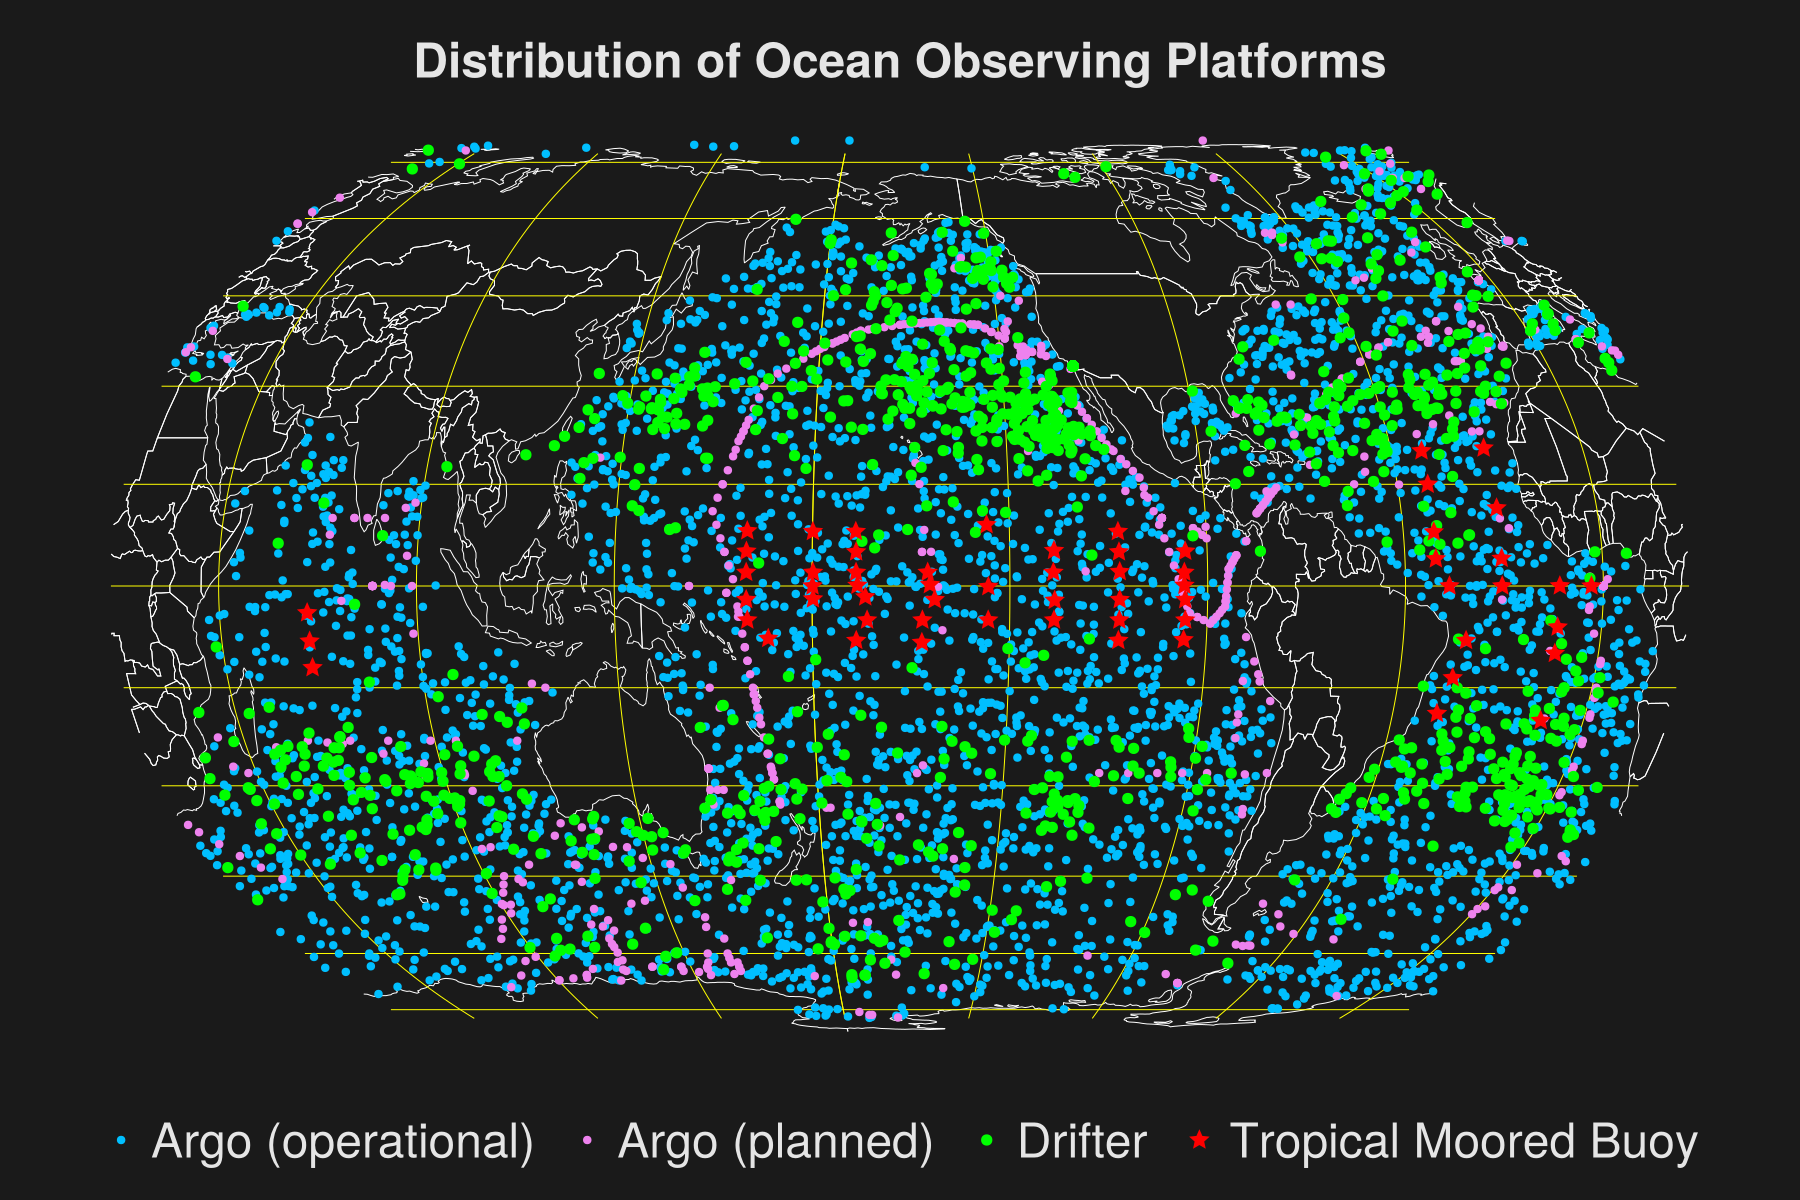
\includegraphics[width=\columnwidth]{figs/20240528_OceanOPS.png}}
\caption{Locations of ocean robots collecting data on {\it 2024/05/27}. Data source : https://www.ocean-ops.org}
\label{fig:ocean-ops}
\end{figure}

\section{Robots Observing the Ocean}

Part of the fleet of ocean robots currently at sea is depicted in Fig.~\ref{fig:ocean-ops}, focusing on a few widely used observing platforms. To create this map, \pkg{OceanRobots.jl} queries the meta-data-base from Ocean-OPS.org, which keeps track of the whole ocean fleet of scientific observing platforms in real time, and provides a RESTful API. The \pkg{OceanRobots.jl} package provides an interface to this API via the `OceanOPS` module. It then defines data structures such as  `SurfaceDrifter` and `ArgoFloat` to access and utilize data from widely used ocean observing platforms. The list of ocean observing platforms currently supported by \pkg{OceanRobots.jl} is in Tab.~\ref{tab:robots}.

\begin{figure}[t]
\centerline{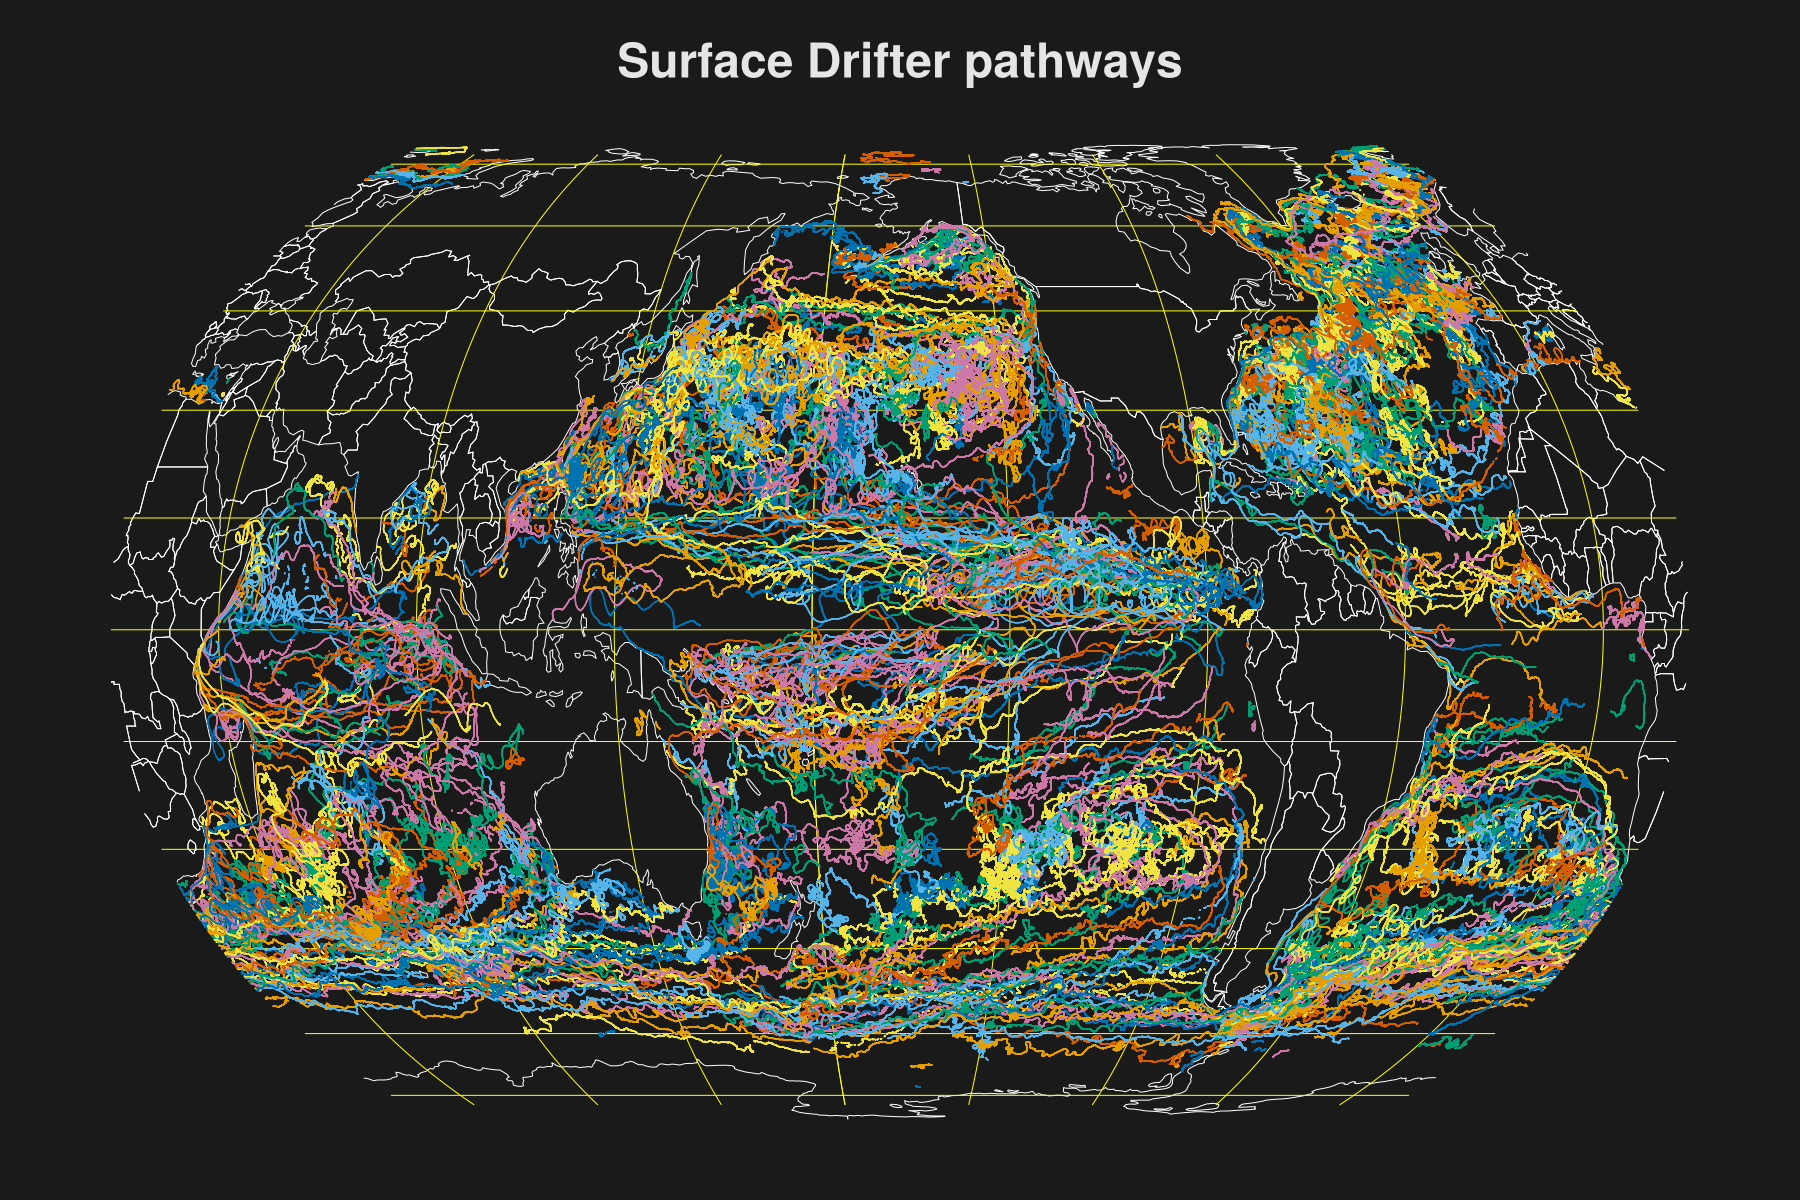
\includegraphics[width=\columnwidth]{figs/20240528_drifters_5percent.png}}
\caption{A few of the ocean drifters (5\% of 19396) that have been deployed to follow near surface ocean currents.}
\label{fig:drifters}
\end{figure}

A fraction of the geospatial data obtained by surface ocean drifters in the past (green dots in Fig.~\ref{fig:ocean-ops}) is depicted in Fig.~\ref{fig:drifters} using \pkg{OceanRobots.jl} and \pkg{Makie.jl}. These drifting buoys tend to follow ocean currents at approximately 15 depth. They can measure sea surface temperature and sea level pressure along their trajectory. The data archive currently holds 19396 drifter trajectories, collected over the past 50 years, which allow us to create climatologies such as the one shown in Fig.~\ref{fig:drifters_ve}.


\begin{table}
\tbl{Ocean observing platforms targeted by \pkg{OceanRobots.jl}, and associated data structures (or blank if not yet implemented).}{
\begin{tabular}{|l||r|}\hline
Platform Type & Data Structure\\\hline\hline
surface drifters & \struct{SurfaceDrifter}, \struct{CloudDrift} \\
drifting profilers & \struct{ArgoFloat} \\
moored buoys & \struct{OceanSite}, \struct{NOAAbuoy} \\
sea gliders & \struct{Gliders} \\
expendable bathy-thermographs & \tbd \\
sail drones & \tbd \\
\hline
research vessel data & \struct{CCHDO} \\
ships of opportunity data & \tbd \\
marine mammals & \tbd \\\hline
\end{tabular}}
\label{tab:robots}
\end{table}

Argo profiling floats (blue dots in Fig.~\ref{fig:ocean-ops}; Code~\ref{lst:ArgoCode}) are one of our main tools to monitor global warming below the sea surface. These devices provide a less detailed view of oceanic pathways (Fig.~\ref{fig:Argo_Float}, top panels) than surface drifters do (e.g., Fig.~\ref{fig:drifters}), since Argo floats only report their location once every ten days. However, Argo floats have a crucial diving capability that surface drifters don't have -- they go up and down the water column to measure temperature and salinity (T,S; bottom panels of Fig.~\ref{fig:Argo_Float}). The advent of the Argo array in the early 2000s \cite{Roemmich2019} thus opened up a whole new era of geospatial analysis, state estimation, and parameter inference over the global Ocean  \cite{Forget2007,Forget2010,MFF14,Forget2015a,FFL15,FP15,Forget2024a}. On `2024/05/27` for example there were 3837 Argo floats at sea, and a total of 18730 in the Argo data base. Since the Argo array is such an important observing system, a dedicated package called \pkg{ArgoData.jl} was created that \pkg{OceanRobots.jl} uses under the hood.

\begin{lstlisting}[
    language = Julia,
%    numbers=left,
    label={lst:ArgoCode},
    caption={Download and visualize one Argo float data as in Fig.~\ref{fig:Argo_Float}.}
]
using OceanRobots, CairoMakie;
argo=read(ArgoFloat(),wmo=6900900);
fig=plot(argo,option=:standard)
\end{lstlisting}

\pkg{OceanRobots.jl} brings these key climate data sets to the Julia community. It provides a bridge to climate scientists working on observations and models, who are interested in leveraging the powerful Julia software ecosystem (e.g., for numerical modeling, machine learning, and statistical analysis), and have much expertise to contribute. The development of \pkg{OceanRobots.jl} aims to help advance (1) how we understand and simulate observations that monitor climate change in the oceans, and (2) climate literacy and education by providing simple apps that anyone can use.

\begin{figure}[t]
\centerline{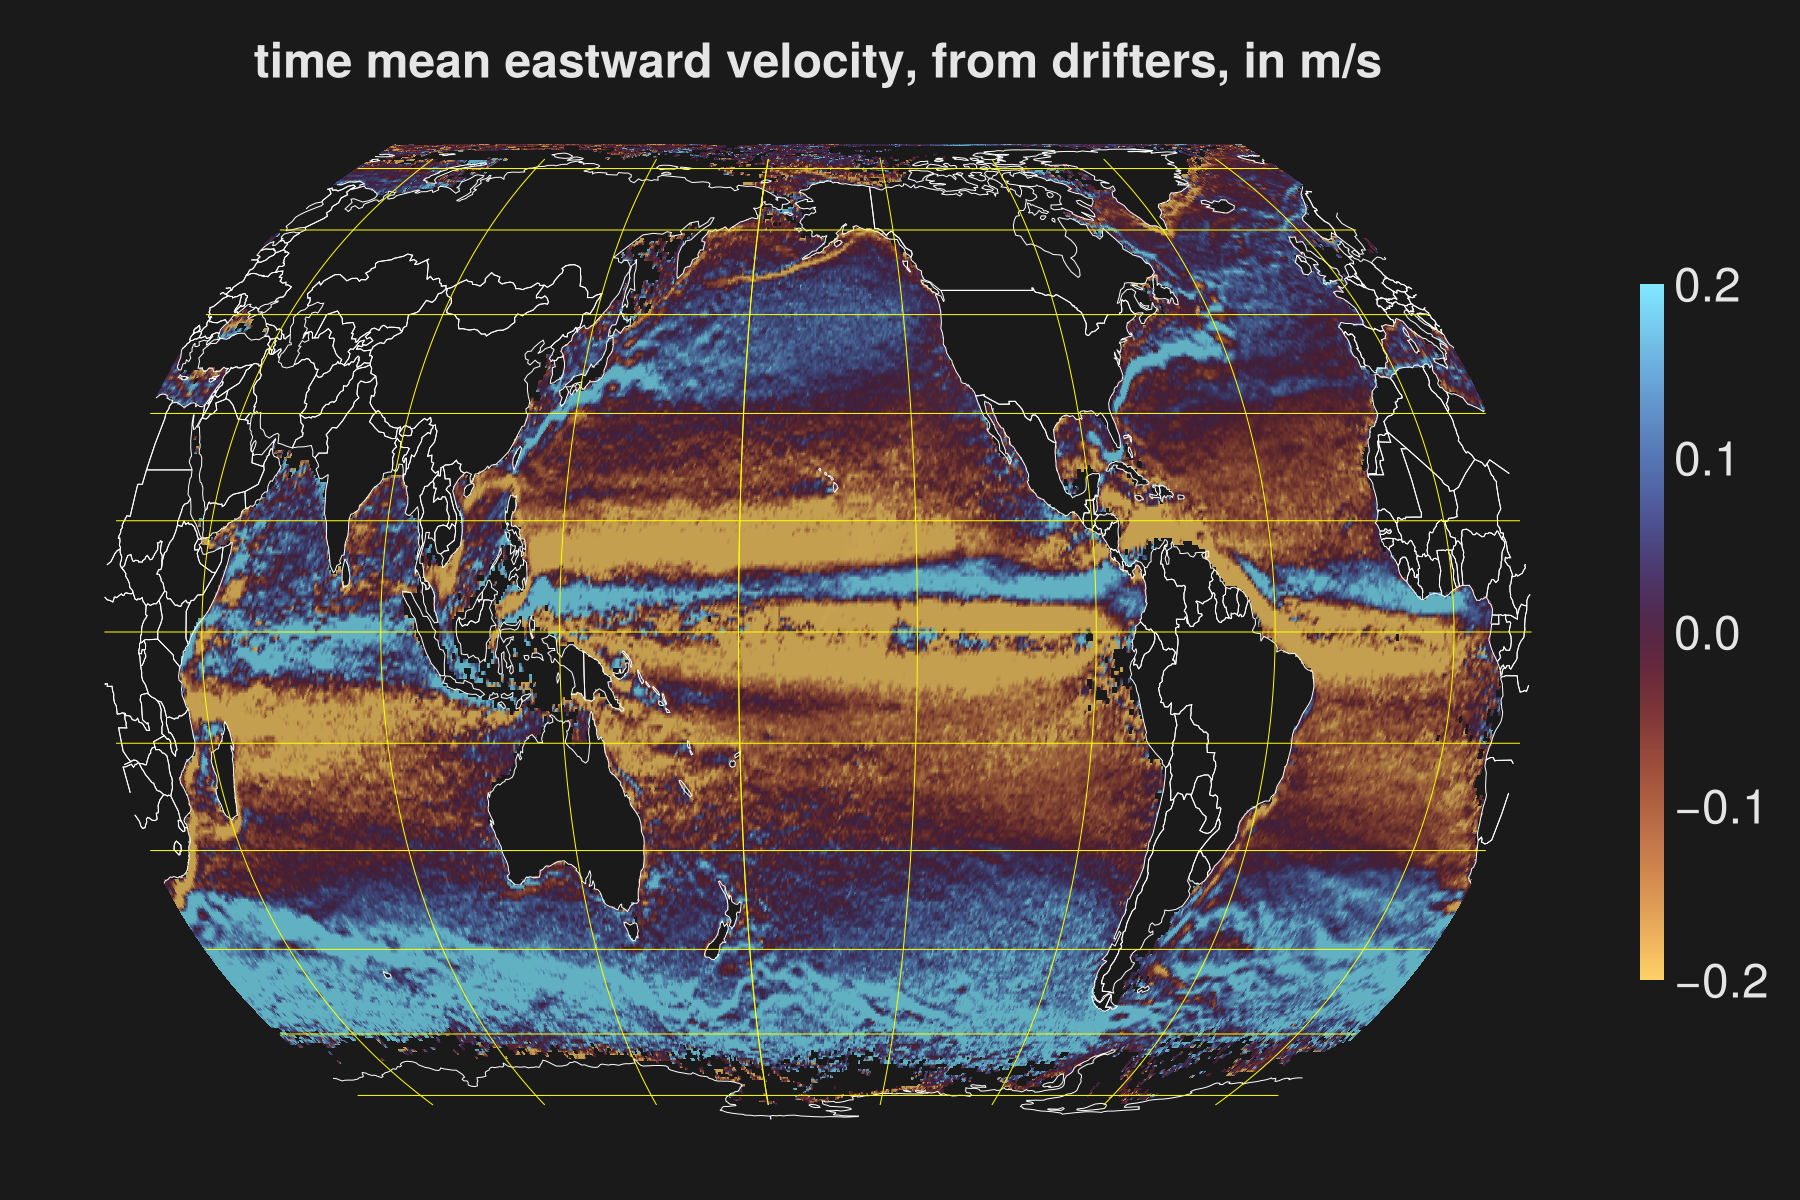
\includegraphics[width=\columnwidth]{figs/20240528_ve_mean.png}}
\caption{Sample mean eastward velocity estimated from drifter data, with a grid resolution of 1/2 degree.}
\label{fig:drifters_ve}
\end{figure}

\section{Simulating Ocean Robots}

Our ability to simulate the data produced by ocean robots is directly linked to our ability, or lack thereof, to explain observed variations and decipher mechanisms from data. Numerical modeling is thus often motivated and driven by observations. Many research activities involve combining ocean models and observations, with the typical goal of learning model parameters, statistics, and dynamics from data \cite{Forget2010,Forget2015a,FFL15,FP15,Forget2024a}. Observing system simulations in a digital environment (using models) enable a wide range of applications -- to test out innovative platform or sensor designs ahead of deployment, to optimize global monitoring strategies, or to guide deployed assets in real time for example.

The two simple examples presented below illustrate the simulation of (1) environmental sensors and (2) observing platforms. First, in Fig.~\ref{fig:Argo_Float_simu} we simulate an Argo data collection for temperature (T) and salinity (S) by sampling an ocean climatology along the track of the Argo float (the one from Fig.~\ref{fig:Argo_Float}). This calculation requires (1) a model prediction of $T(x,y,z,t)$ and $S(x,y,z,t)$, which can be based on statistical or mechanistic models on a grid, and (2) tools that deal with the Earth geography, and can localize observations on a grid, and perform interpolation tasks. 

To create Fig.~\ref{fig:Argo_Float_simu}, we use \pkg{Climatology.jl} to access the OCCA climatology \cite{Forget2010}, and then interpolate $T(x,y,z,t)$, $S(x,y,z,t)$ via geospatial tools from \pkg{MeshArrays.jl}. The OCCA climatology is a previously trained model that consists of 12 monthly three-dimensional fields of $T,S$ (one per calendar month). The fact that Figs.~\ref{fig:Argo_Float} and~\ref{fig:Argo_Float_simu} show broadly similar patterns reflects that the predictive model is skillful, and that $T,S$ contrasts seen in Fig.~\ref{fig:Argo_Float} largely result from the sensor moving with the Argo float across the Ocean's $T,S$ geography. Differences between Figs.~\ref{fig:Argo_Float} and~\ref{fig:Argo_Float_simu} can in turn provide a basis for improving the predictive model, for example by including time variability beyond the seasonal cycle, or through various methods for data assimilation, artificial intelligence, or parameter inference \cite{Forget2010,Forget2015a,FFL15,FP15,Forget2024b}.

\begin{figure}[t]
\centerline{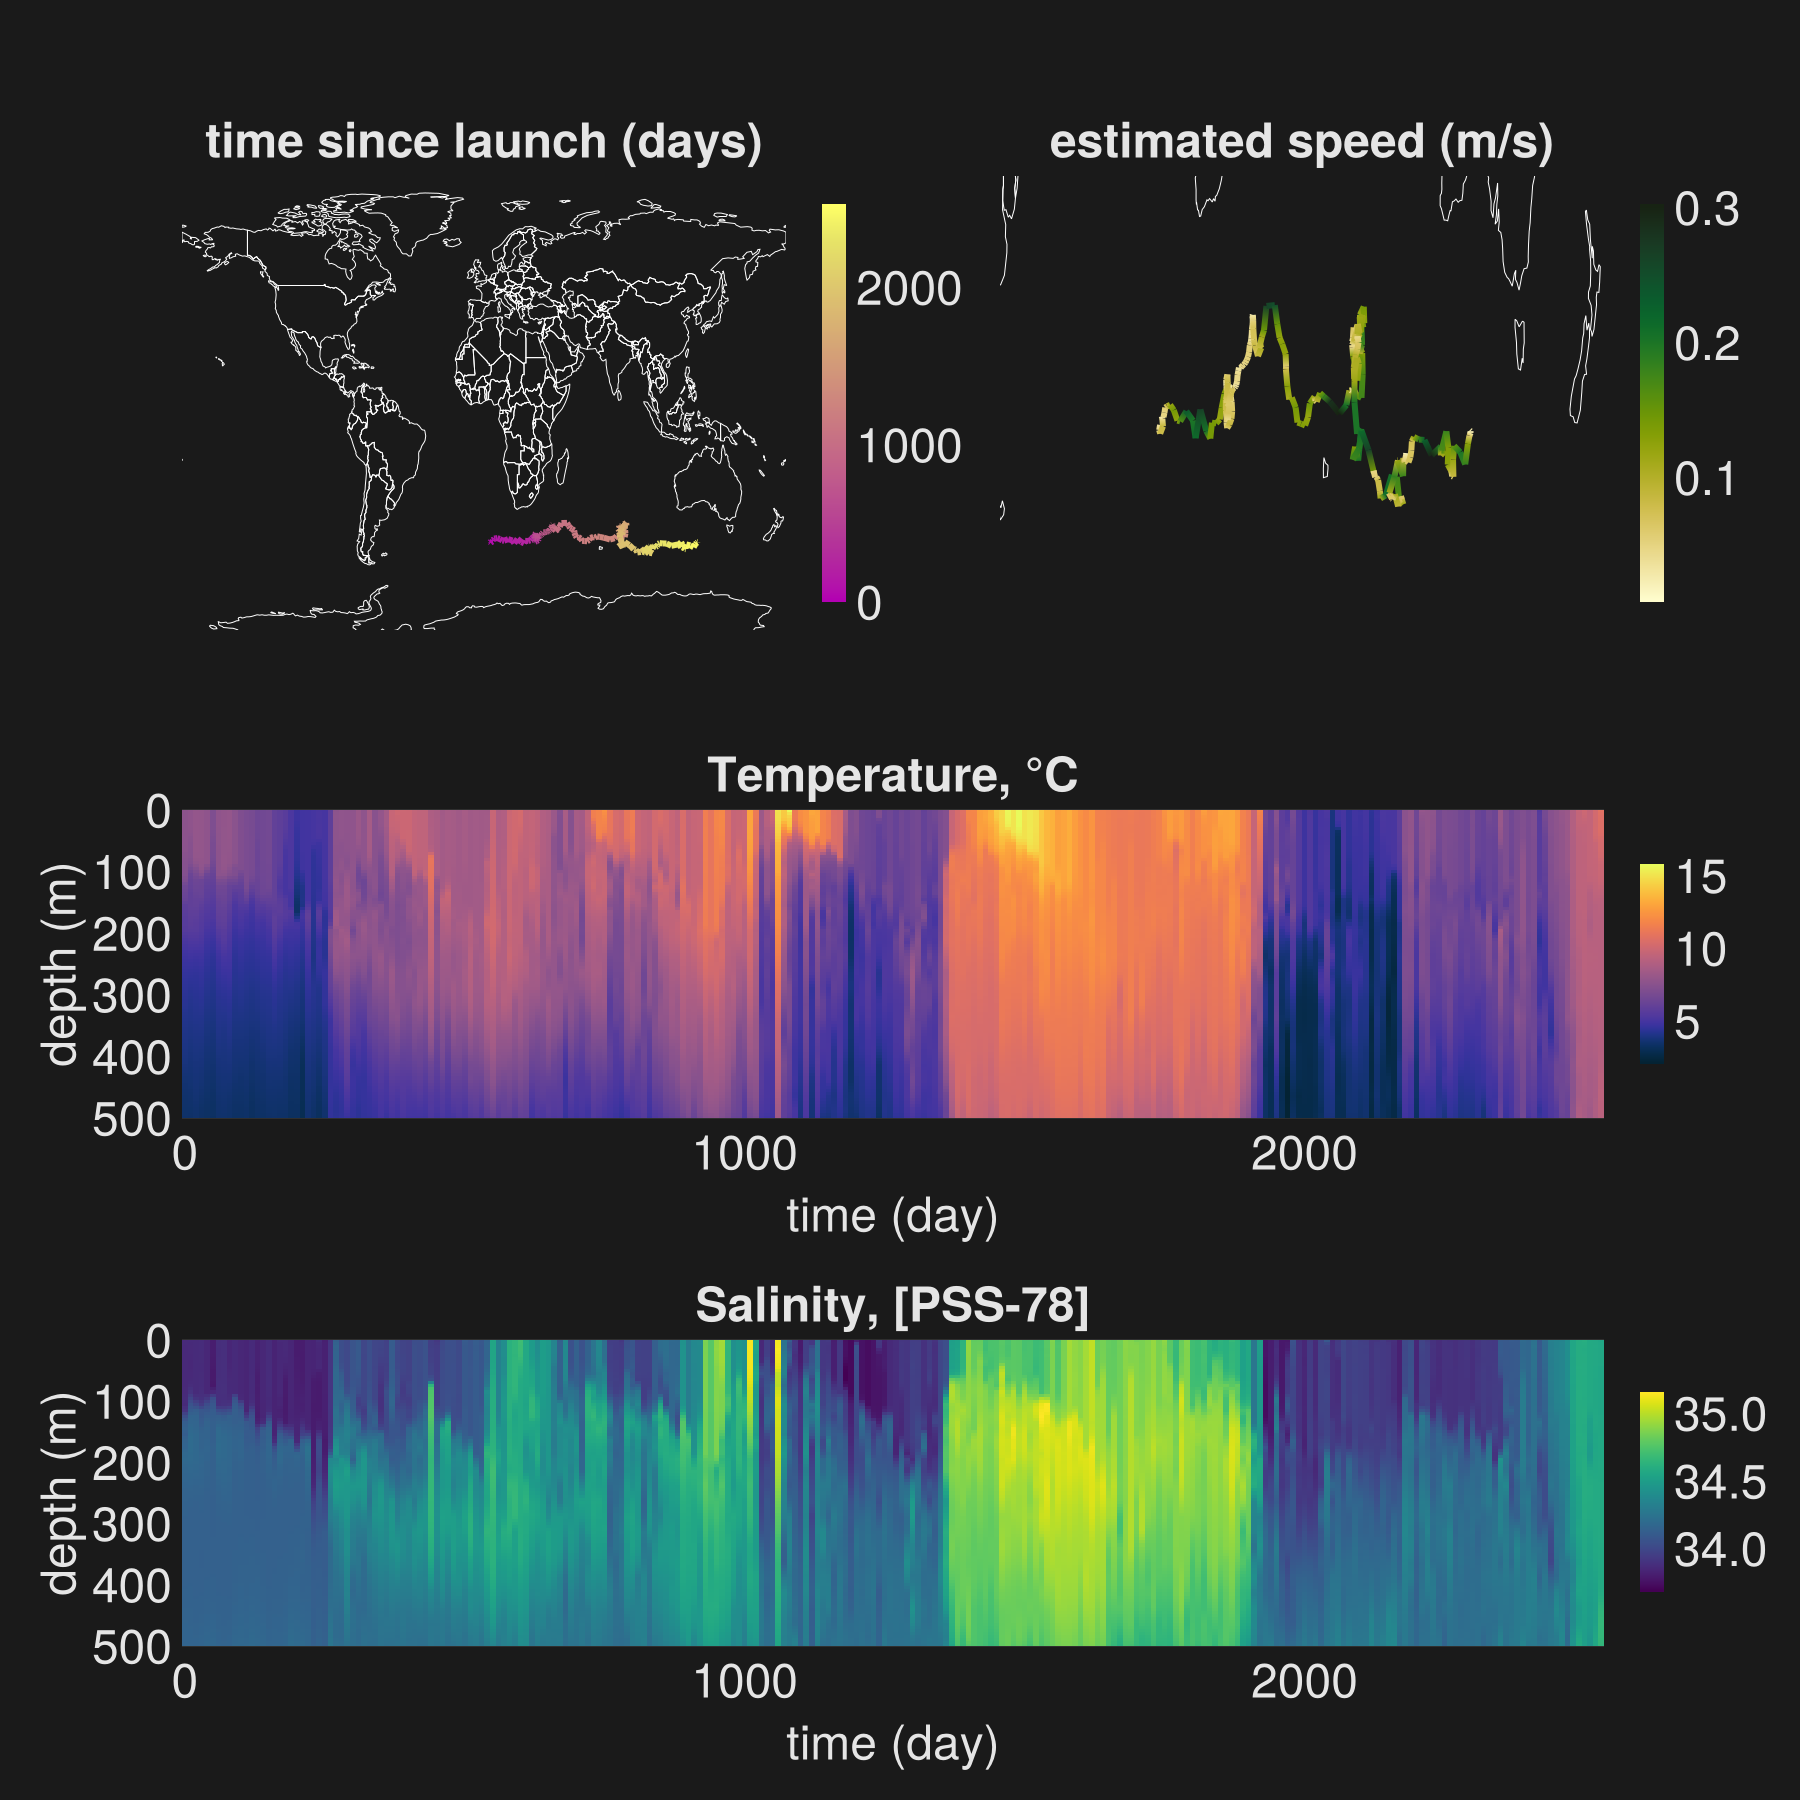
\includegraphics[width=\columnwidth]{figs/20240528_Argo_6900900.png}}
\caption{Data collected by a profiling float from the Argo array. Temperature and salinity profiles, taken every ten days, extend to 2000m depth.}
\label{fig:Argo_Float}
\end{figure}

\begin{figure}[t]
\centerline{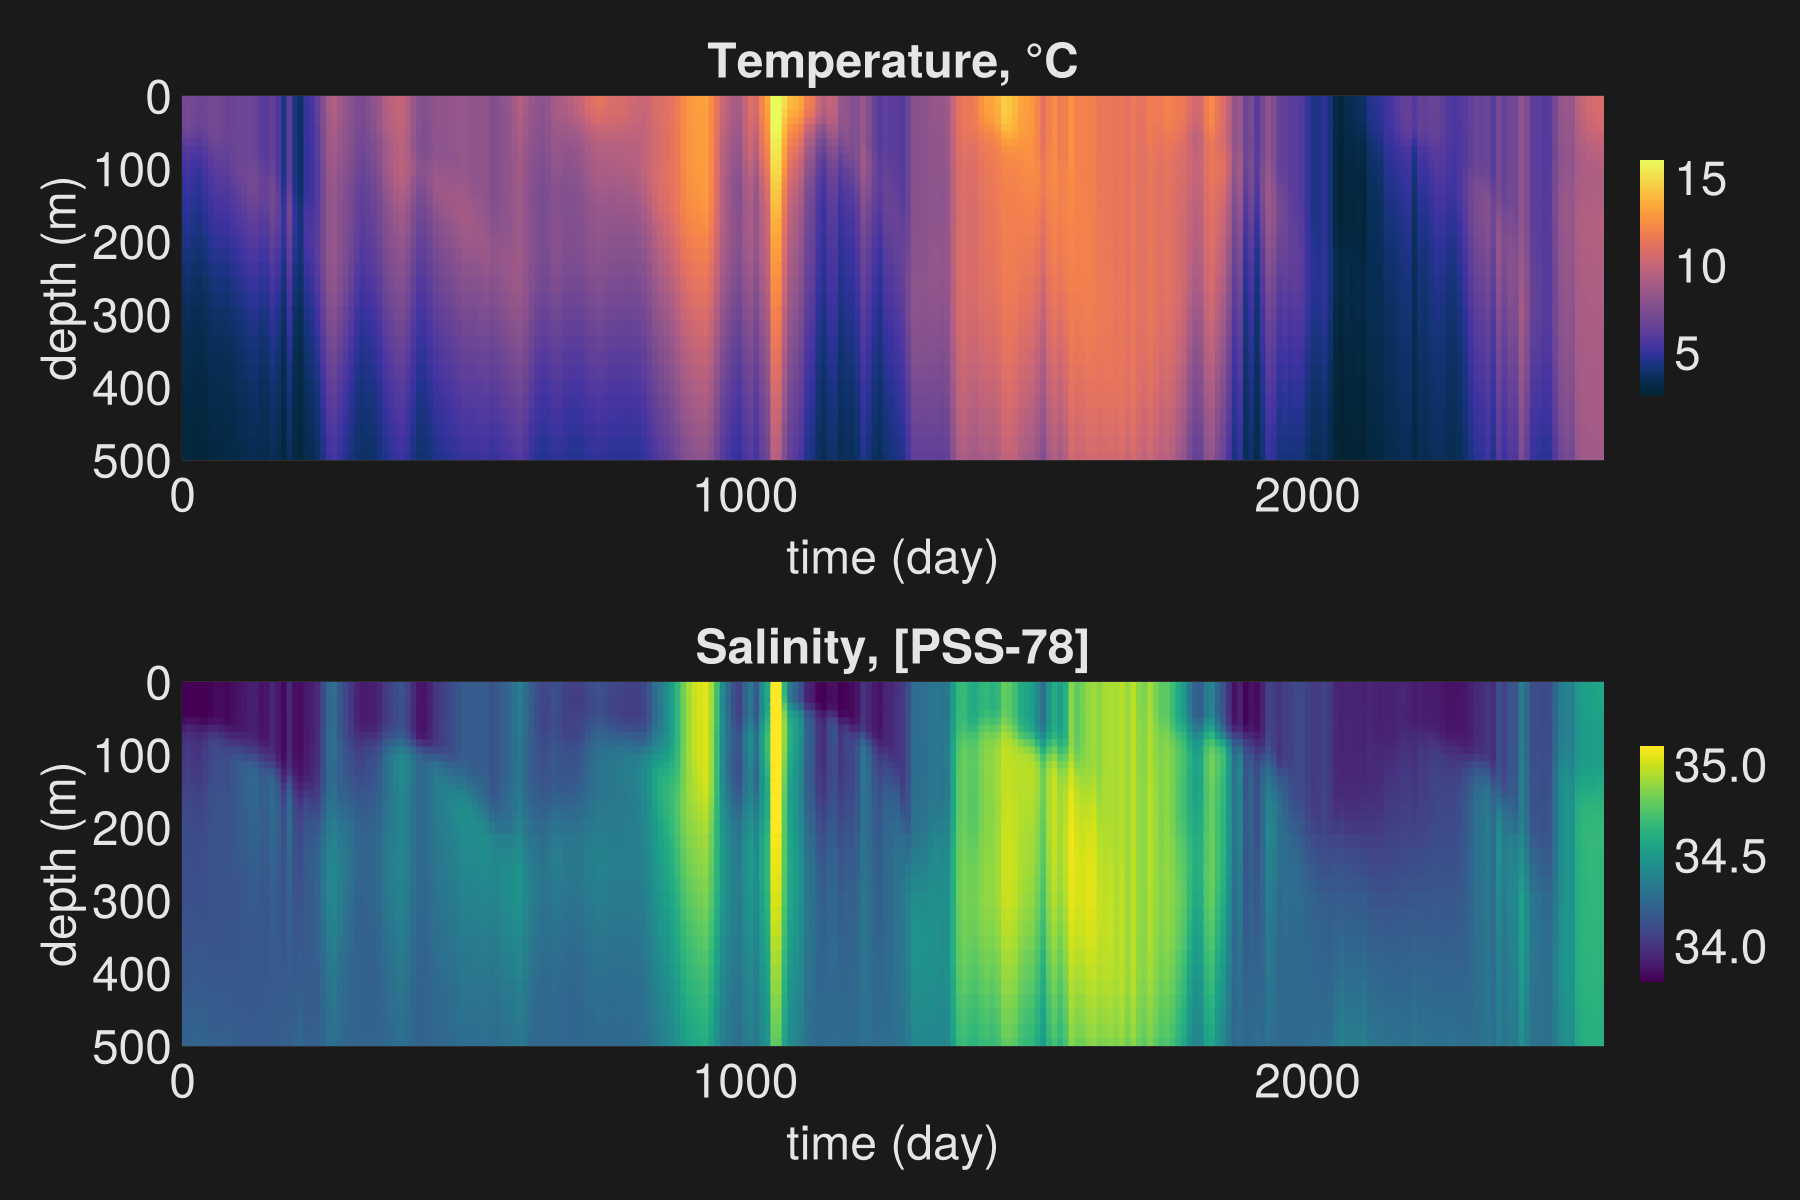
\includegraphics[width=\columnwidth]{figs/20240529_MITprof_OCCA.png}}
\caption{Virtual Argo profiles predicted using the OCCA climatology, interpolated to the positions of the float shown in Fig.~\ref{fig:Argo_Float}.}
\label{fig:Argo_Float_simu}
\end{figure}

Our second example focuses on the simulation of observing platforms moving with ocean currents. This basic simulation of surface drifter pathways uses the geostatistical average of velocities calculated in Fig.~\ref{fig:drifters_ve} as a predictive model for the $U(x,y,t)$, $V(x,y,t)$ velocity fields. In Code~\ref{lst:IndDispCode}, this gridded data set is provided as input to \pkg{Drifters.jl}, which then releases virtual drifters and calculates their trajectories following the flow field (Fig.~\ref{fig:drifters_speed_simu}). While this simple drifter trajectory prediction model neglects stochastic variability and small scales in ocean currents altogether (Fig.~\ref{fig:km_scale}), it is sufficient to capture the main mean pathway of sea water through the Gulf of Mexico region -- the well-known loop current feeding the Gulf Stream via Florida Strait (Fig.~\ref{fig:drifters_speed_simu}).

Much more could be done to improve the details and skill of the simple models used here. Higher-order and higher-resolution model output are available to represent important aspects of what is being observed, but neglected in Figs.~\ref{fig:Argo_Float_simu} and~\ref{fig:drifters_speed_simu}, such as the turbulent dispersion seen in Fig.~\ref{fig:drifters_speed} or the small-scale variations visible in Fig.~\ref{fig:Argo_Float}. Small scale temperature fronts and currents are present everywhere in the ocean, with a lot of heterogeneity across regions, as illustrated in Fig.~\ref{fig:km_scale}. Hence it is important to include global km-scale ocean simulations in our model hierarchy (see section~\ref{sec:DT}). 

\begin{figure}[t]
\centerline{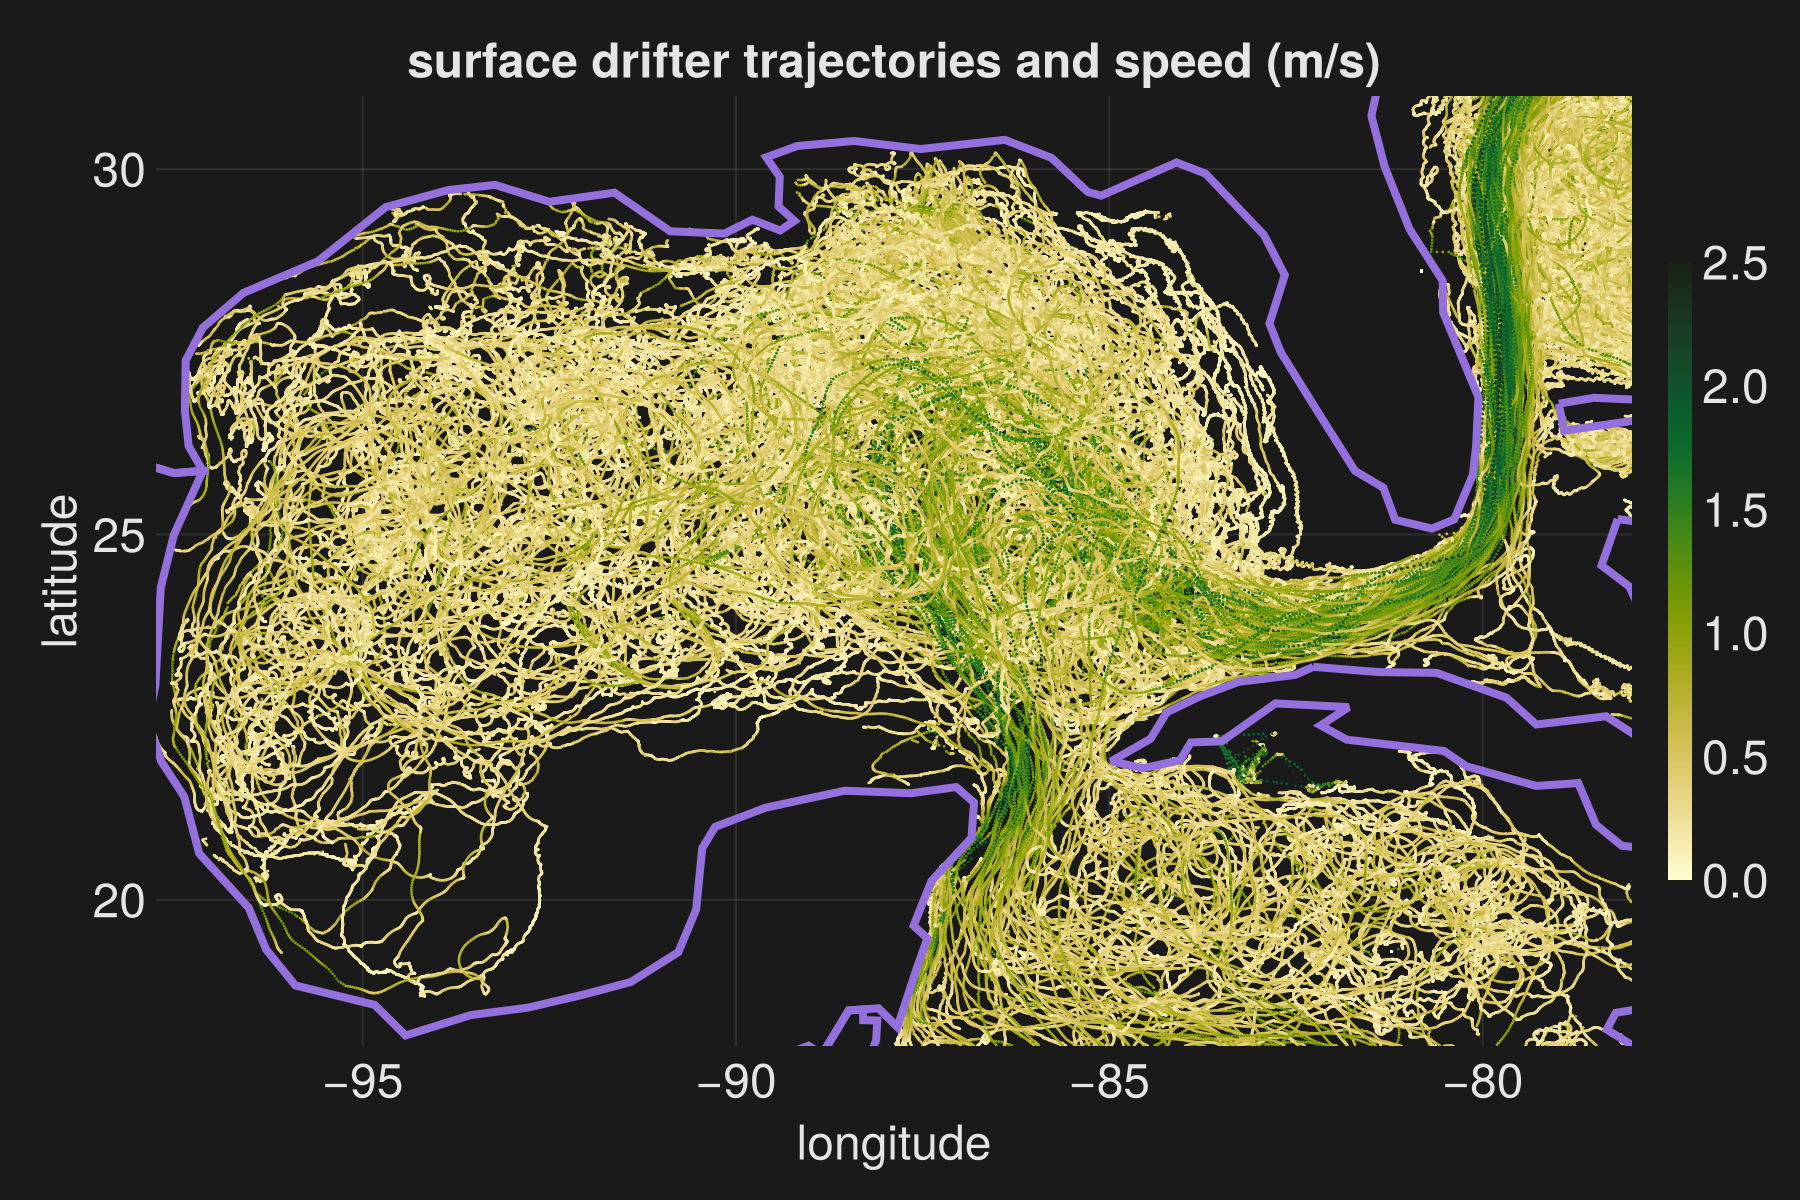
\includegraphics[width=\columnwidth]{figs/20240528_speed_subset.png}}
\caption{Drifter trajectories in the Gulf of Mexico region. Large velocities highlight the path of the Gulf Stream, being fed by the loop current.}
\label{fig:drifters_speed}
\end{figure}

\begin{figure}[t]
\centerline{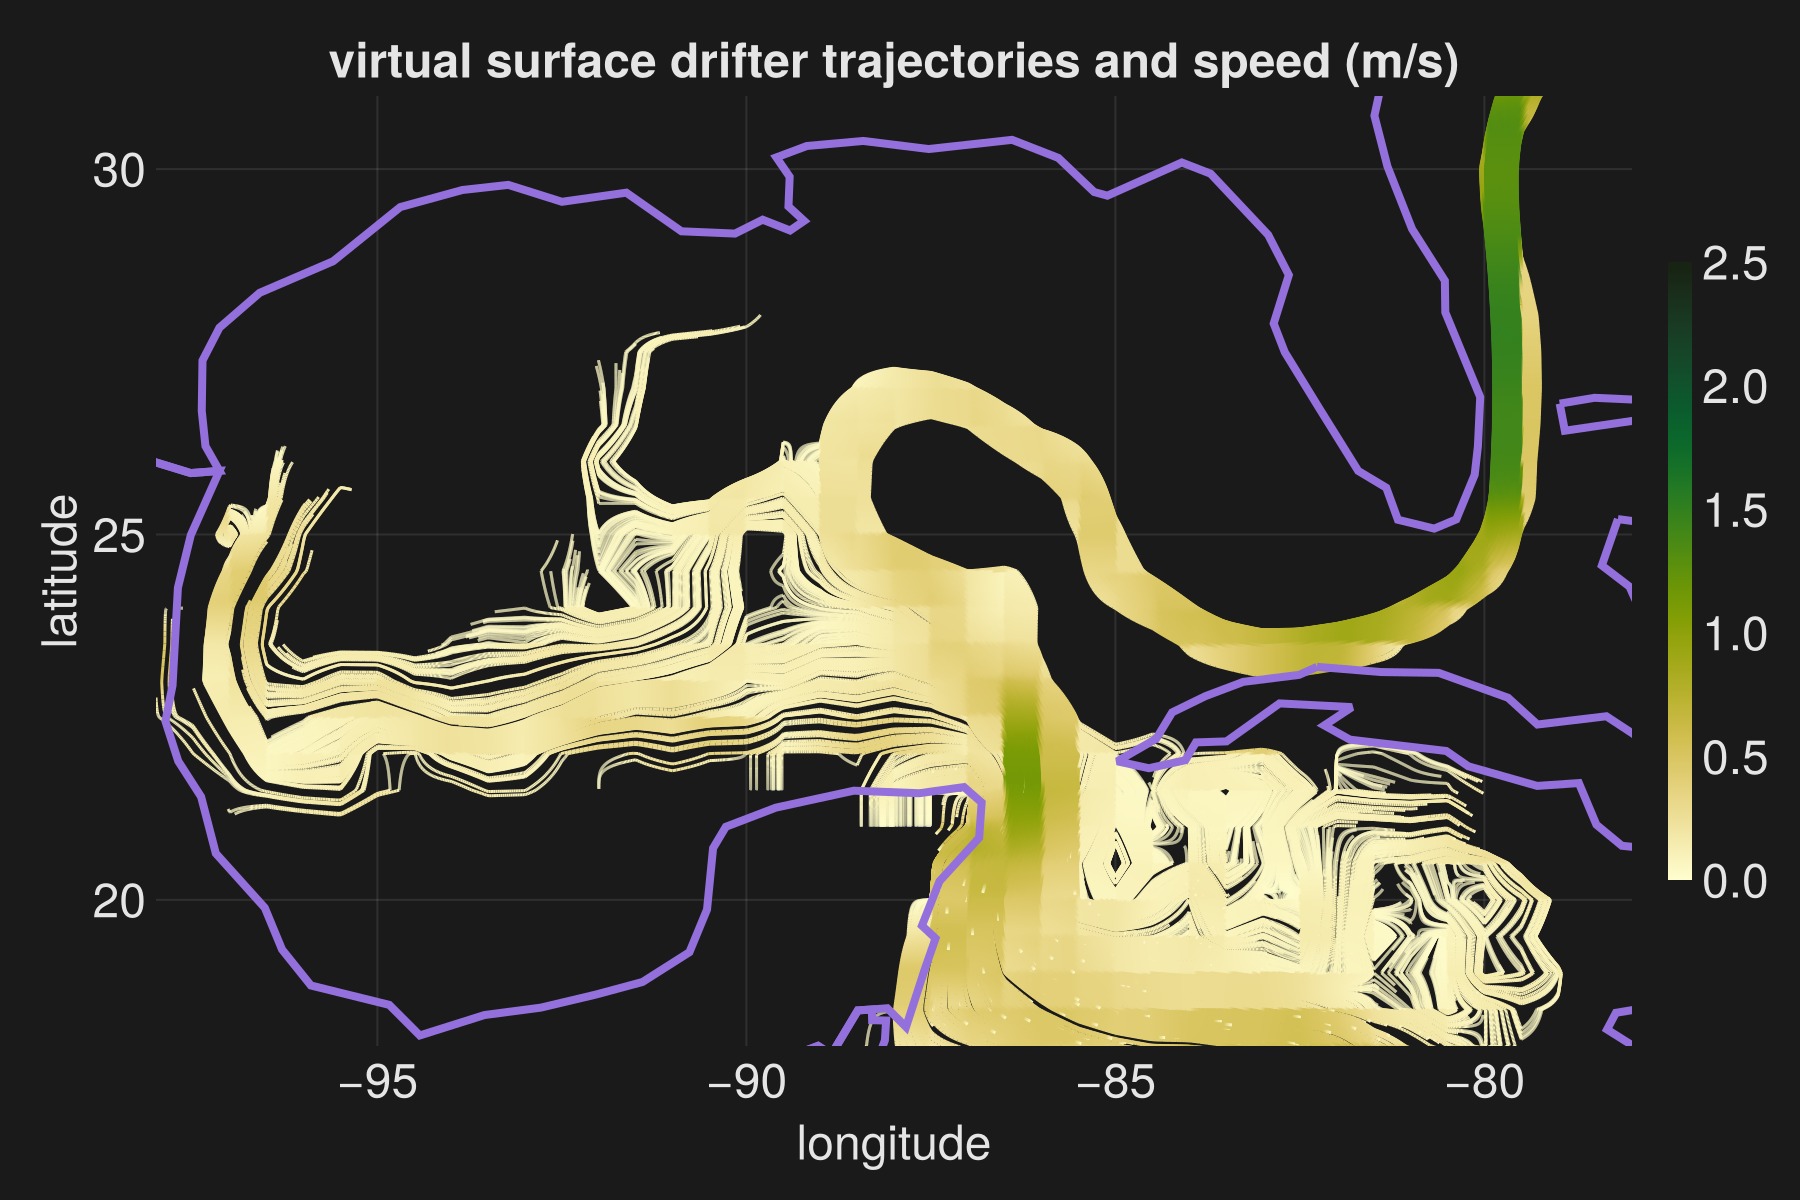
\includegraphics[width=\columnwidth]{figs/20240529_speed_subset_IndDisp.png}}
\caption{Virtual drifter trajectories predicted using (1) just the climatological mean flow field estimated from drifters (Fig.~\ref{fig:drifters_ve}, and the northward component) and (2) \pkg{Drifters.jl} to calculate trajectories.}
\label{fig:drifters_speed_simu}
\end{figure}


\begin{lstlisting}[
    language = Julia,
    label={lst:IndDispCode},
    caption={Simulate surface drifter pathways in the Gulf of Mexico (Fig.~\ref{fig:drifters_speed}) from flow fields $u,v$ and initial positions $x,y$. 
    Visualization code is provided in the \pkg{Drifters.jl} documentation.}
]

using OceanRobots, Drifters, CairoMakie ;
P=Drifters.Gulf_of_Mexico_setup();
F=FlowFields(u=P.u,v=P.v,period=P.T);
I=Individuals(F,P.x0,P.y0);
[solve!(I,P.T .+P.dT*(n-1)) for n in 1:P.nt];
\end{lstlisting}

\section{Digital Twin Framework} \label{sec:DT}

Let's define digital twins as agreed upon by the U.S. Committee on Foundational Research Gaps and Future Directions for Digital Twins \cite{DT2024} : 

\begin{defi}
A digital twin is a set of virtual information constructs that mimics the structure, context, and behavior of a natural, engineered, or social system (or system-of-systems), is dynamically updated with data from its physical twin, has a predictive capability, and informs decisions that realize value. The bidirectional interaction between the virtual and the physical is central to the digital twin.
\end{defi}

In the {\it digital twins for ocean robots} framework (DTOR), interactivity is facilitated by Julia and its large ecosystem of software packages. In particular, \pkg{Makie.jl} \cite{Makie} and \pkg{Pluto.jl} \cite{Pluto} let us operate even complex modeling workflows from notebooks and apps. The tutorial examples in \pkg{OceanRobots.jl}, \pkg{ArgoData.jl}, \pkg{ClimateModels.jl}, and \pkg{MITgcm.jl} \cite{Forget2024b} are notably available as Pluto notebooks. Interaction between model and data is further enabled by the rich Julia ecosystem for machine learning, data assimilation, parameter inference, etc. Fig.~\ref{fig:MLP} provides an example where \pkg{Flux.jl} \cite{Innes2018} is used to train neural networks to predict chlorophyll concentration (linked to marine microbe abundance) from environmental parameters as done in the CANYON model \cite{Sauzede2017,Bittig2018}.

The core of DTOR is formed by \pkg{OceanRobots.jl}, \pkg{ArgoData.jl}, and \pkg{MeshArrays.jl} for the physical twins, along with \pkg{Climatology.jl}, \pkg{ClimateModels.jl}, \pkg{MITgcm.jl}, and \pkg{Drifters.jl} for the virtual twins (i.e., predictive modeling). The \pkg{ClimateModels.jl} interface streamlines the use of models implemented in various languages. The model hierarchy already includes the models used in this paper, and is easy to extend via pkg{ClimateModels.jl}. DTOR can notably simulate observations in the future based on climate model predictions, and \pkg{ClimateModels.jl} provides two options for this kind of applications -- either querying the CMIP6 archive of model output \cite{CMIP6} or using a fast emulator such as Hector \cite{Hector2015} (Fig.~\ref{fig:globalwarming}). 

Within our model hierarchy, future climate scenarios like Fig.~\ref{fig:globalwarming} can be downscaled using gridded climatologies and reanalyses \cite{Forget2010,Forget2015a,Forget2024a}. The ECCO4 and OCCA2 reanalyses are simple to rerun with perturbed surface forcing fields via \pkg{MITgcm.jl}, which is particularly convenient for such applications. Multi-decadal solutions produced in this way can then be further downscaled using km-scale model output (Fig.~\ref{fig:km_scale}). At the end of this modeling workflow, \pkg{OceanRobots.jl}, \pkg{MeshArrays.jl} and \pkg{Drifters.jl} enable calculations such as Figs.~\ref{fig:Argo_Float_simu} and \ref{fig:drifters_speed_simu}, for any of our models. DTOR can also take advantage of gridded satellite data, incl. sea surface temperature and sea level anomalies via \pkg{Climatology.jl}, and it is sometimes possible to use these instead of ocean reanalyses.

\begin{figure}[th]
\centerline{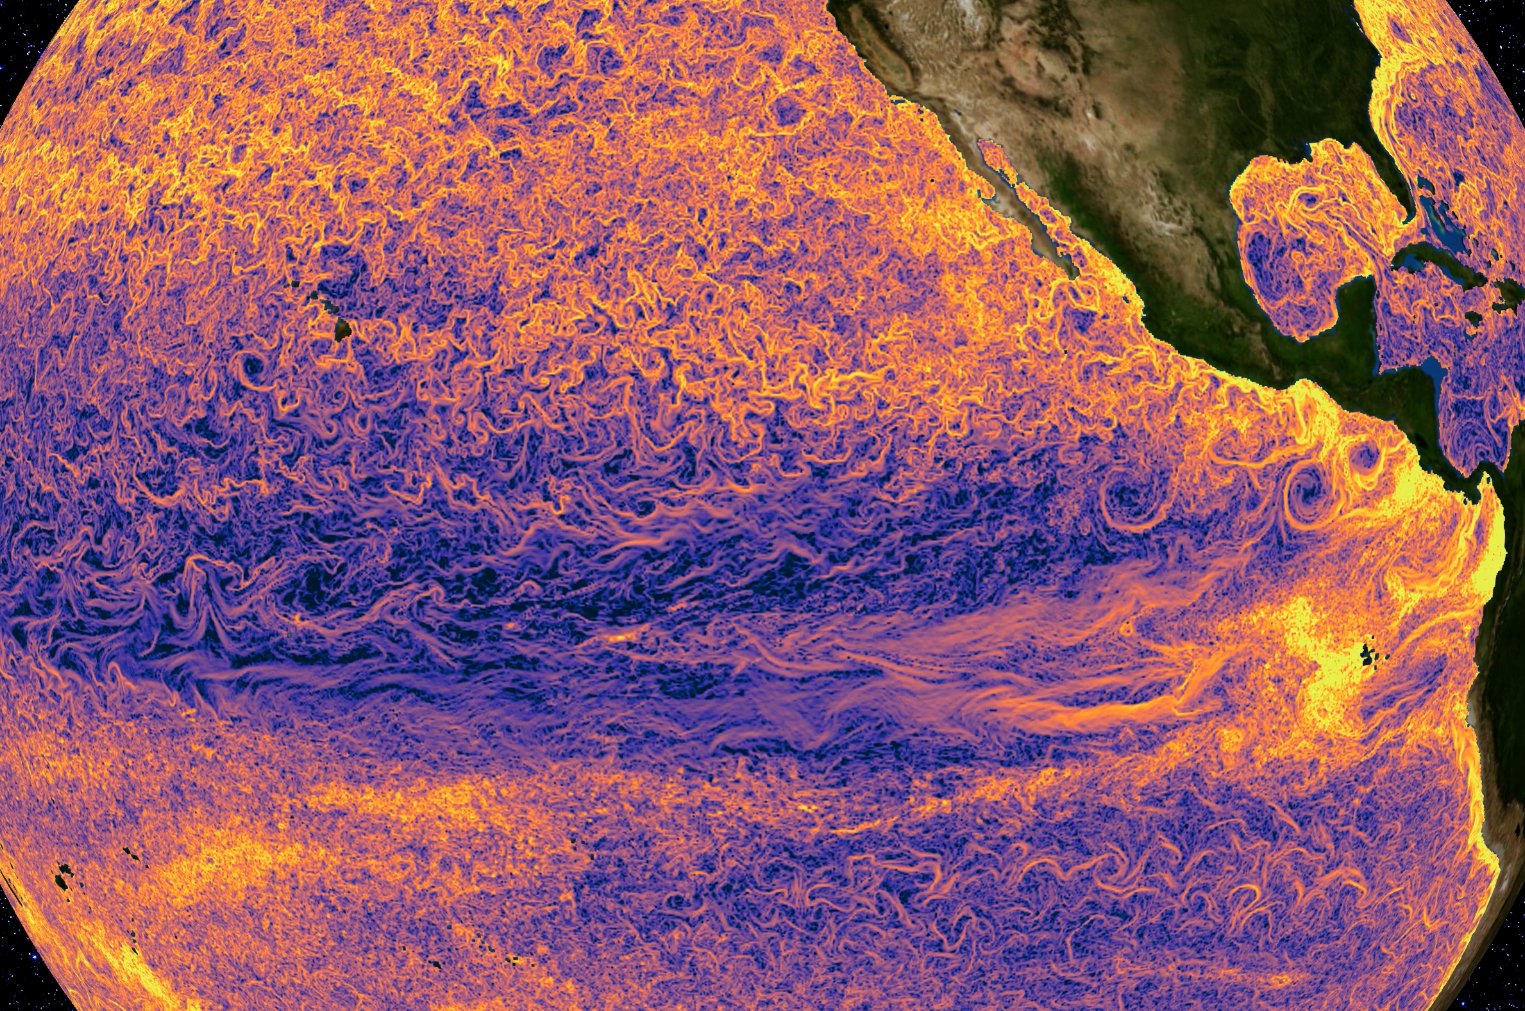
\includegraphics[width=\columnwidth]{figs/Snapshot_grad_theta.png}}
\caption{Temperature fronts in a global km-scale MITgcm simulation. Plotted is the logarithm of the spatial gradient of a temperature snapshot.}
\label{fig:km_scale}
\end{figure}

\begin{figure}[th] 
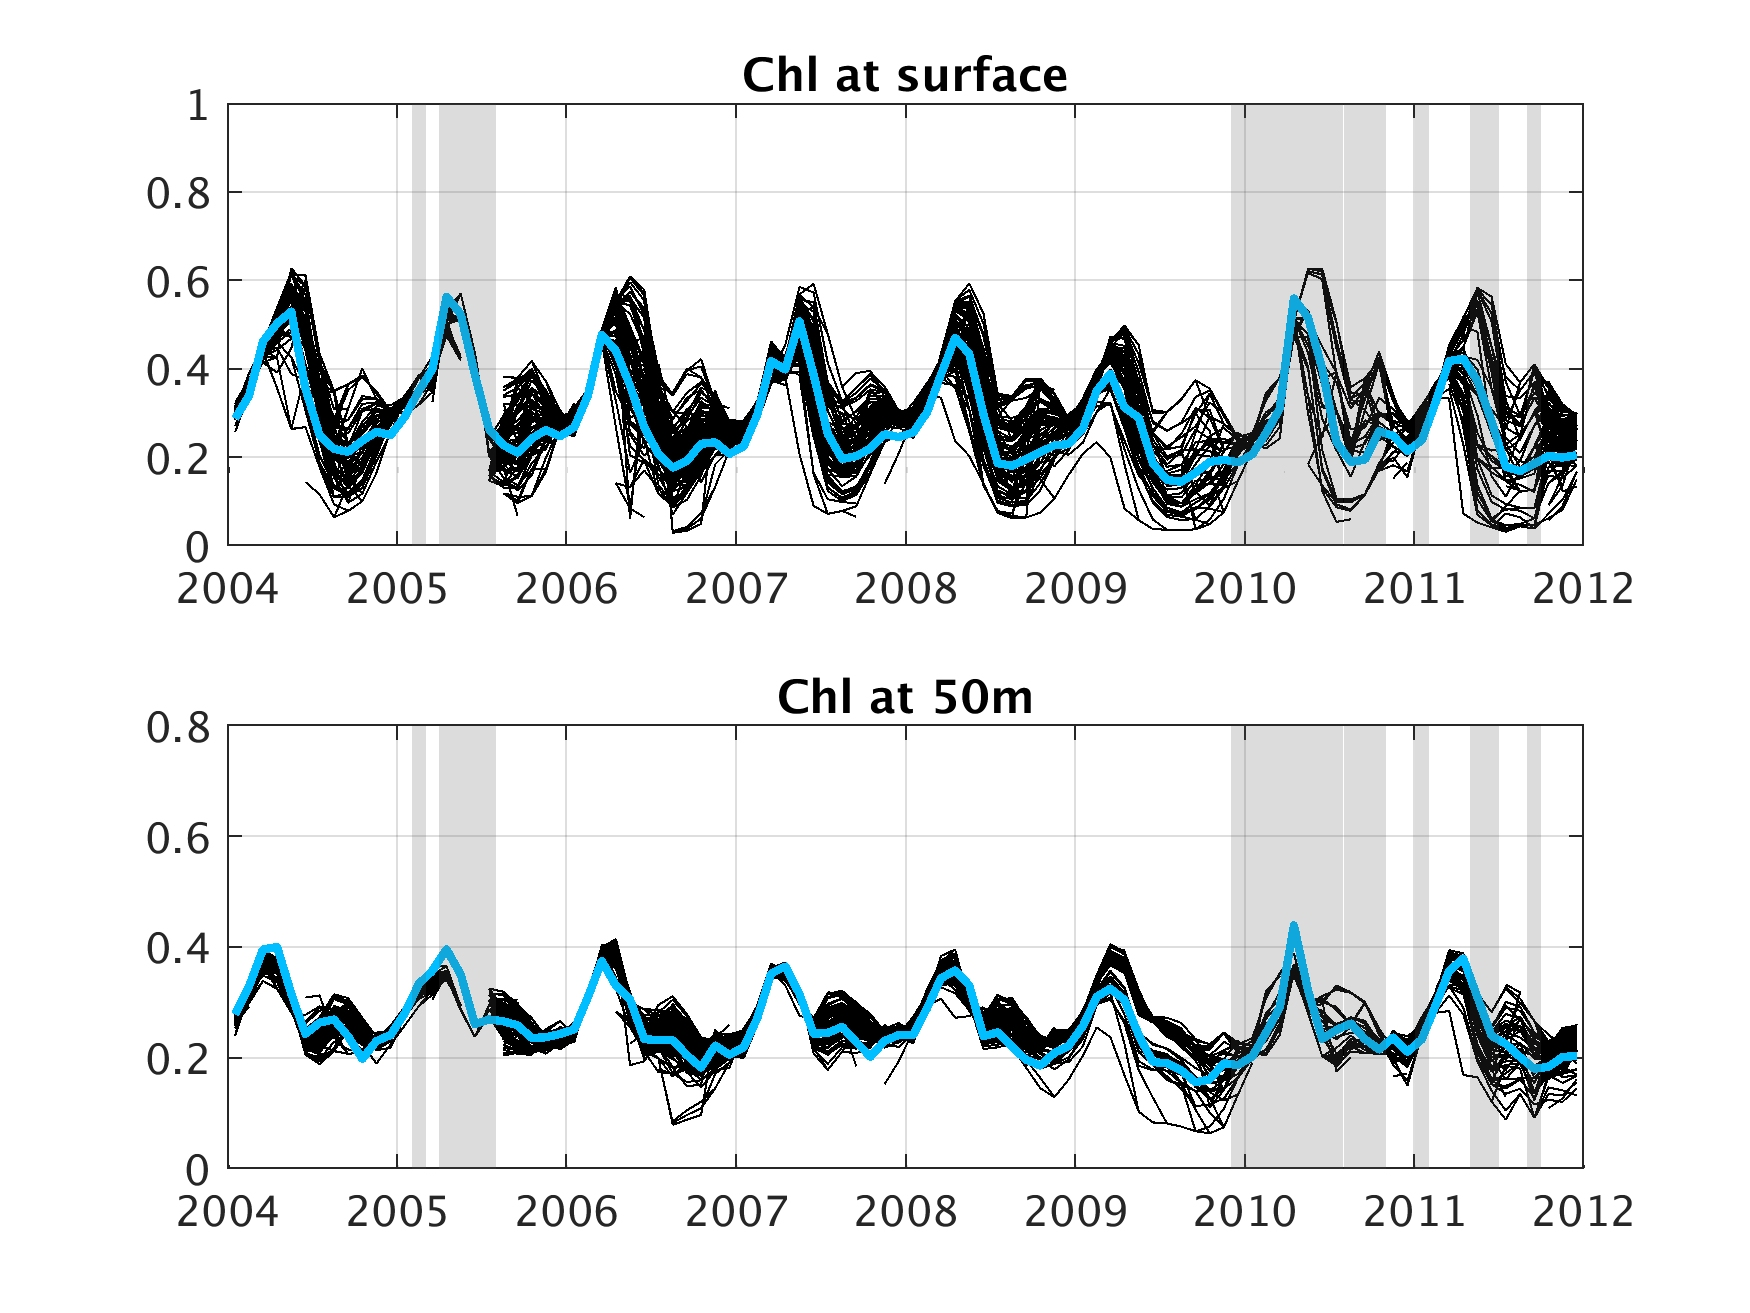
\includegraphics[width=\columnwidth]{figs/Chl_av_NN3D5.jpg}
\caption{Ensemble of model predictions (black curves) by a simple multi-layer perceptron (from Flux.jl) trained to predict Chlorophyll concentration (present in green algea and marine microbes) from environmental variables (T, S, but also oxygen, optical backscatter, and solar radiation). The blue line is the {\it ground truth} that we seek to estimate, and was obtained through proper spatial averaging of the gridded data set from which the training data itself was generated.}
\label{fig:MLP}
\end{figure} 

\begin{figure}[th] 
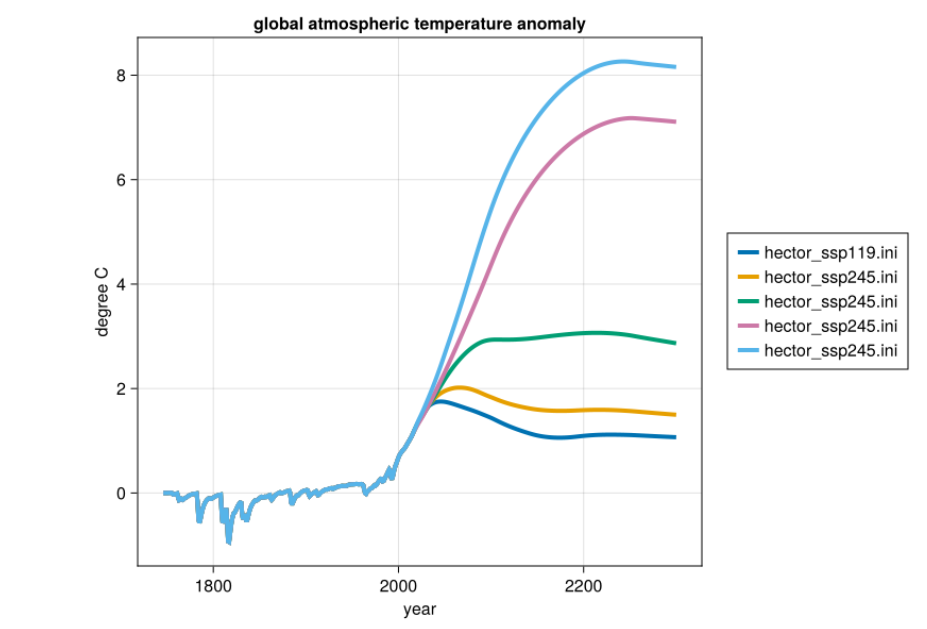
\includegraphics[width=\columnwidth]{figs/HectorDemo.png}
\caption{Prediction of global warming based on different scenarios, called Shared Socioeconomic Pathways (SSPs), as defined by the Intergovernmental Panel on Climate Change (IPCC). These predictions were generated using the Hector model \cite{Hector2015} via \pkg{ClimateModels.jl}.}
\label{fig:globalwarming}
\end{figure} 

\section{Planned Extensions}

Further development of the DTOR framework is expected to proceed in several directions. First, we'd like to integrate additional types of ocean observing platforms, starting with those that do not have a data structure listed yet in Tab.~\ref{tab:robots}. Observational networks that focus on either the coastal ocean, a specific region, or local field experiments could be supported in the future. A top level API to interact with DTOR as a whole through cloud services is also envisioned.

A second direction to pursue is that of further integration with the Julia software stack. Ocean modeling capabilities such as \pkg{Oceananigans.jl} \cite{OceananigansJOSS}, \pkg{PlanktonIndividuals.jl} \cite{Wu2022}, \pkg{AIBECS.jl} \cite{Pasquier2022}, \pkg{OceanColorData.jl}, and \pkg{WorldOceanAtlasTools.jl} are of immediate relevance. More broadly, there is a lot of very useful work being done across of number of github organizations that DTOR could further leverage and integrate with. To list a few : \pkg{JuliaClimate}, \pkg{JuliaOcean}, \pkg{CLIMA}, \pkg{JuliaGeo}, \pkg{JuliaEarth}, \pkg{JuliaSpace}, \pkg{JuliaRobotics}, \pkg{juliadynamics}, \pkg{MakieOrg}, \pkg{PlutoOrg}, \pkg{JuliaHub}, \pkg{GenieFramework}, \pkg{JuliaStats}, \pkg{SciML}, \pkg{FluxML}, \pkg{Turing}, and \pkg{JuliaAI}. 

\section{Science Applications}

Our current focus is on geospatial analyses that track global warming and marine heatwaves using Argo data \cite{Forget2024a}. Another example from our research is with the C-Streams observational program (UK-US) which is releasing drifters near Florida Strait to track the nutrient stream that is associated with the Gulf Stream. A simulation of these pathways is shown in Fig.~\ref{fig:Cstream}, which is based on the monthly mean ECCO4 climatology for ocean transports \cite{Forget2015a,Forget2019,Rousselet2021}, and uses \pkg{Climatology.jl}, \pkg{MeshArrays.jl}, and \pkg{Drifters.jl} to calculate pathways. Other applications at the scale of oceanic basins include tracking ocean plastic pollution, monitoring biological impacts of extreme events and global warming, or the optimization of the global climate monitoring fleet of ocean robots. DTOR could be used to pilot field experiments (e.g., S-MODE, to choose an example from the recent past). Related projects on digital twins, not focused on exploiting Julia but interested in ocean observations, include the EU funded {\it Destination Earth} program, Mercator Ocean International's {\it Digital Twin Ocean}, and the UN Decade Action's DITTO initiative ({\it Digital Twins of The Ocean}).

\begin{figure}[hb] 
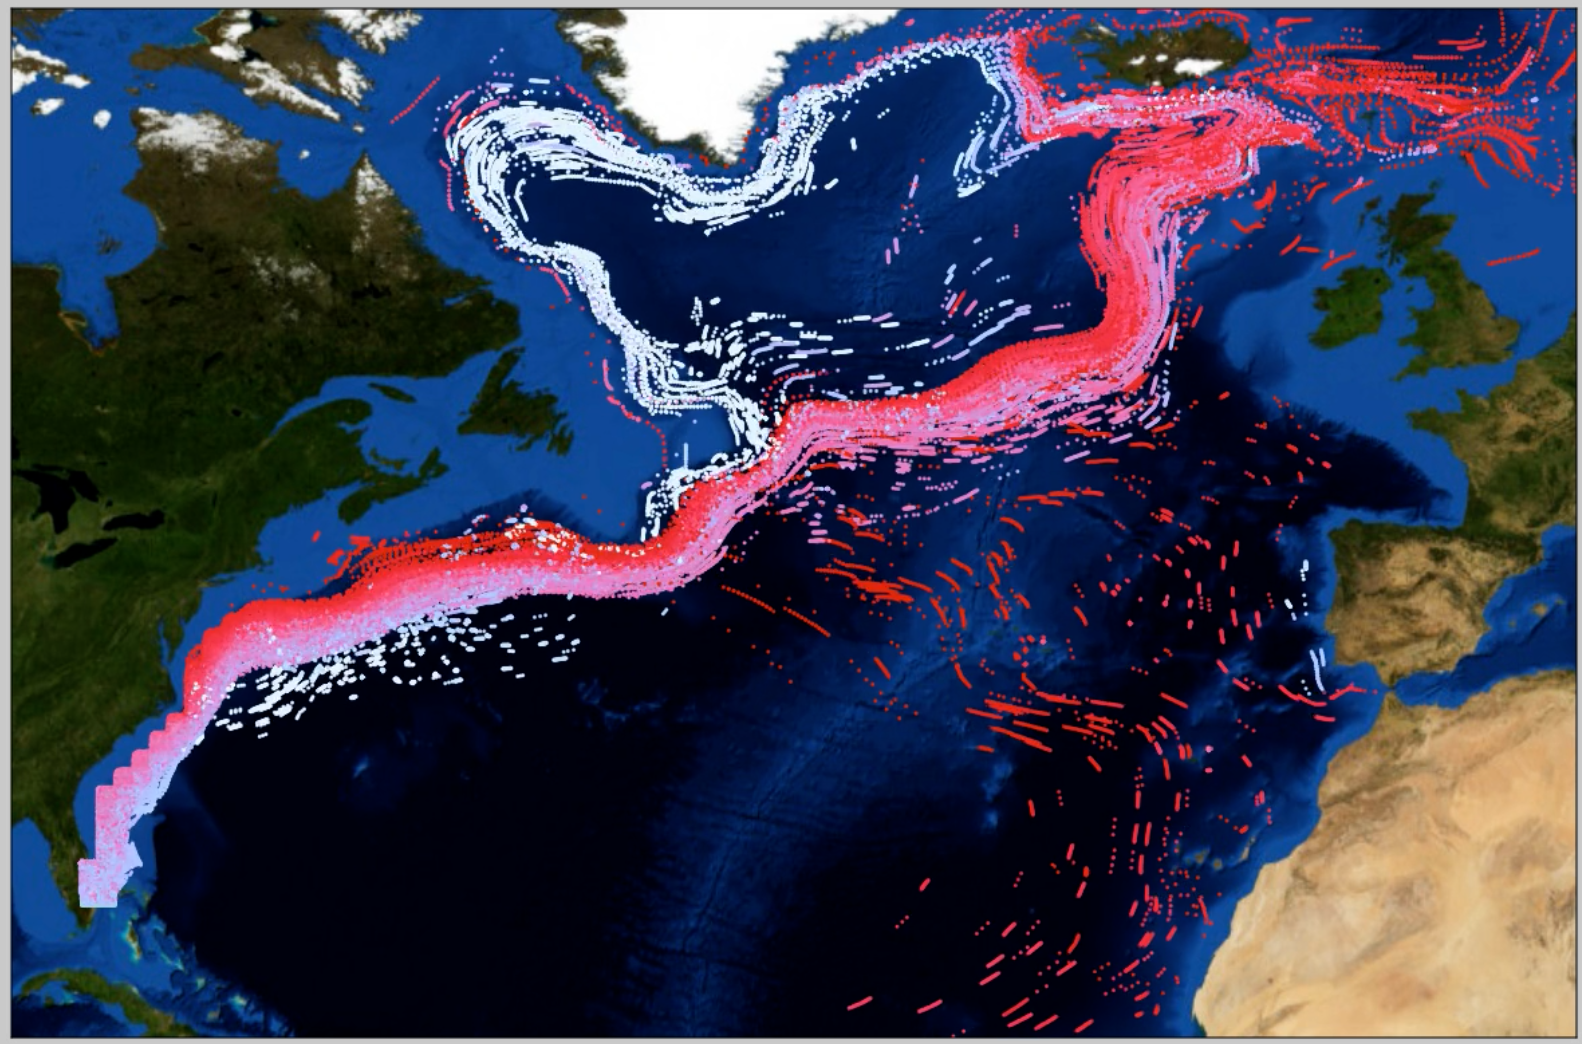
\includegraphics[width=\columnwidth]{figs/GulfStream_21_27_snapshot.png}
\caption{Tracking Gulf Stream waters from Florida Strait to the subpolar gyre using virtual drifters that follow the three dimensional ocean circulation. Each dot color indicates the virtual drifter depth -- red dots near the sea surface, while white dots are below 1500m depth.}
\label{fig:Cstream}
\end{figure} 

\section{Acknowledgements}

Support from NASA awards 80NSSC20K0796, 80NSSC23K0355, 80NSSC22K1697, 1676067, and 1686358, as well as from the Simons Foundation via the CBIOMES and SCOPE-GRADIENTS program is acknowledged for this work.

% **************GENERATED FILE, DO NOT EDIT**************

\bibliographystyle{juliacon}
\bibliography{ref.bib}


\end{document}
